\documentclass[../main/main.tex]{subfiles}

\newdate{date}{14}{10}{2020}

% \begin{figure}[h!]
% \centering
% \includegraphics[page=6,width=0.8\textwidth]{../lessons/pdf_file/08_lecture.pdf}
% \end{figure}

%\displaydate{date}. Compiled:  \today. Alice.

\begin{document}

\pagestyle{plain}

\section{Lecture 8}


\subsubsection*{Slide 1}

\begin{minipage}[]{0.5\linewidth}
\centering
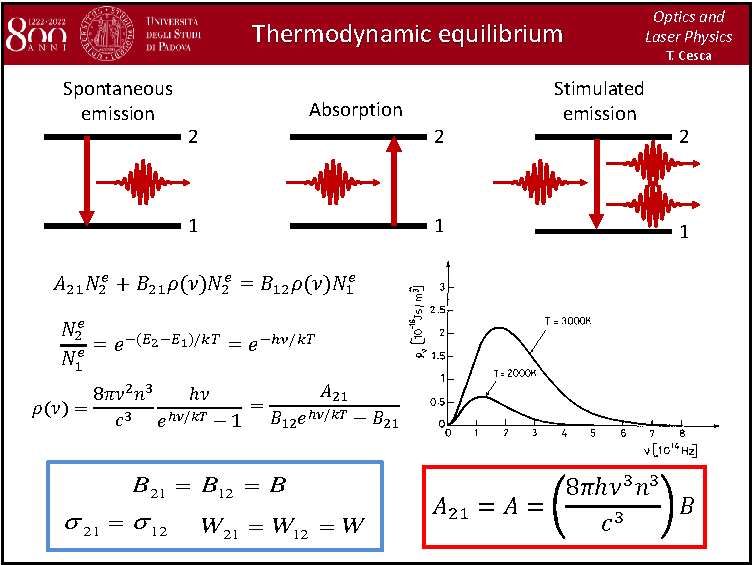
\includegraphics[page=1,width=1\textwidth]{../lessons/pdf_file/08_lecture.pdf}
\end{minipage}
\hspace{0.3cm}
\vspace{0.3cm}
\begin{minipage}[c]{0.47\linewidth}

There is an elegant demonstration by Einstein whose exploit thermodynamic to calculate the three decay rates for the three processes.

We have a material embedded in a black blody. At thermodynamic equilibrium, we have a balance between spontaneous emission, absorption and stimulated emission.
The first two term on the lhs are the one of spontaneous and stimulated emission. The term on the rhs is the one off absorption.

At thermodynamic equilibrium, we have also the Boltzmann statistic for the population of the two levels.

It is easy to obtain the energy density as this expression. In order to satisfy this equality, we have that the Einstein coefficient for stimulated emission should be equal to absoprtion and so on.

\end{minipage}

We have also a relation between the spontaneous emission \( A \) and the absorption (or stimulated emission) \( B \).

\( n \) is the refractive index of the medium. We have a term \( \nu ^3 \): the spontaneous emission will dominate for very high frequency. At UV every material become fluerescent.

These results are valid for non degenerate levels.

\subsubsection*{Slide 2}

\begin{minipage}[]{0.5\linewidth}
\centering
\includegraphics[page=2,width=1\textwidth]{../lessons/pdf_file/08_lecture.pdf}
\end{minipage}
\hspace{0.3cm}
\vspace{0.3cm}
\begin{minipage}[c]{0.47\linewidth}

In the degenerate case, we have to take into account the degeneracy \( g_1 \) and \( g_2 \) of level 1 and 2.
However, the physics of the process does not change.

\end{minipage}

\subsubsection*{Slide 3}

\begin{minipage}[]{0.5\linewidth}
\centering
\includegraphics[page=3,width=1\textwidth]{../lessons/pdf_file/08_lecture.pdf}
\end{minipage}
\hspace{0.3cm}
\vspace{0.3cm}
\begin{minipage}[c]{0.47\linewidth}

Until now, we have considered a semi-classical approach. If you want to adopt a more formal quantum mechanical approach, we have to introduce \textbf{Fermi's golden rule} in order to describe the decay rate for one of these processes.

The transition rate can be written as a function of the \textbf{local density of final optical states (LDOS)}.

The transition matrix should be written as the integral of the Hamiltonian.

\end{minipage}

\newpage

\subsubsection*{Slide 4}

\begin{minipage}[]{0.5\linewidth}
\centering
\includegraphics[page=4,width=1\textwidth]{../lessons/pdf_file/08_lecture.pdf}
\end{minipage}
\hspace{0.3cm}
\vspace{0.3cm}
\begin{minipage}[c]{0.47\linewidth}

We can use different Hamiltonian and so we have different kind of transitions.

The most probable transition is the \textbf{Electric-dipole transition (E1)}: the Hamiltonian is written as
\begin{equation*}
  H' = - \va{p} \cdot \va{E}
\end{equation*}
We think the two level system as a dipole. We have the interaction of the dipole and the electric field of the beam.

The term \( \mu_{12}  \) take into account the characteristic of the level we are considering and \( E \) is the electric field of the beam.

\end{minipage}

\subsubsection*{Slide 5}

\begin{minipage}[]{0.5\linewidth}
\centering
\includegraphics[page=5,width=1\textwidth]{../lessons/pdf_file/08_lecture.pdf}
\end{minipage}
\hspace{0.3cm}
\vspace{0.3cm}
\begin{minipage}[c]{0.47\linewidth}

The probability of electric-dipole transition is strongest wrt others. However, we have also other transitions.

We can consider also higher order transitions.

Actually, the higher is the order, the lower is the transition rate. That is why these system from a quantum mechanic point of view are described by dipoles.


\end{minipage}

\subsubsection*{Slide 6}

\begin{minipage}[]{0.5\linewidth}
\centering
\includegraphics[page=6,width=1\textwidth]{../lessons/pdf_file/08_lecture.pdf}
\end{minipage}
\hspace{0.3cm}
\vspace{0.3cm}
\begin{minipage}[c]{0.47\linewidth}

Making the exact calculation for the transition E1, it is possible to obtain the exact value for the Einstein coefficient \( A_{21} \) (spontaneous emission) and \( B_{21} \) (stimulated emission equal to absoprtion if we are not considering degenerate levels).

Einstein could determine the ratio
\begin{equation*}
  \frac{A}{B} = \frac{8 \pi h \nu ^3 n^3}{c^3}
\end{equation*}
well in advance wrt a quantum mechanical approach.

\end{minipage}

\newpage

\subsubsection*{Slide 7}

\begin{minipage}[]{0.5\linewidth}
\centering
\includegraphics[page=7,width=1\textwidth]{../lessons/pdf_file/08_lecture.pdf}
\end{minipage}
\hspace{0.3cm}
\vspace{0.3cm}
\begin{minipage}[c]{0.47\linewidth}

Just for completness, by considering the degeneracy of the levels, we have to consider the different quantum number for the level.

The \textbf{oscillator's strength} take into account the amplitude of the different transition. It is related to the different strength of the process of the transition. Indeed, the transition are not the same in terms of amplitude.

\end{minipage}

\subsubsection*{Slide 8}

\begin{minipage}[]{0.5\linewidth}
\centering
\includegraphics[page=8,width=1\textwidth]{../lessons/pdf_file/08_lecture.pdf}
\end{minipage}
\hspace{0.3cm}
\vspace{0.3cm}
\begin{minipage}[c]{0.47\linewidth}

The different transitions have to obey to different \textbf{selection rules}: we have allowed and forbidden transition.

If you have a \emph{forbidden transition} does not mean that you never get that transition, but it means that (you have to think in term of probability) they have a very low probability to occur.

The oscillator strength depends also on the selection rules and on the fact that the transition is allowed or forbidden.

\end{minipage}

\subsubsection*{Slide 9}

\begin{minipage}[]{0.5\linewidth}
\centering
\includegraphics[page=9,width=1\textwidth]{../lessons/pdf_file/08_lecture.pdf}
\end{minipage}
\hspace{0.3cm}
\vspace{0.3cm}
\begin{minipage}[c]{0.47\linewidth}

The transition rate (probability for a transition to occur) is not an intrinsinc property of a material. The \emph{interaction matrix element} depends only on intrinsic properties, however the transition rate \textbf{depends} also on the \emph{local density of final states}.

So, by changing the local density, you can control the transition rate!

The plot show that it is possible to modulate the lifetime for spontaneous emission by modifing the local density of final state. In the paper a mono layer of a material containing emitters is considered.
It is on top of a \emph{spacer} such that it as a distance from a mirror.

By changing the relative distance of the spacer, in this paper is shown that the lifetime (and a consequence the radiative decay rate) is changed. So, what is doing in this paper is changin the local density of final states, nothing else.

\end{minipage}

\subsubsection*{Slide 10}

\begin{minipage}[]{0.5\linewidth}
\centering
\includegraphics[page=10,width=1\textwidth]{../lessons/pdf_file/08_lecture.pdf}
\end{minipage}
\hspace{0.3cm}
\vspace{0.3cm}
\begin{minipage}[c]{0.47\linewidth}

The possibility to control the liftime of an emitter is interesting for many applications. Let us consider Erbium in Silica. Erbium is used for optical communication (optical fiber). It can be excited with a light beam in the visible and it emits in a range which minimize the losses in optical fiber.

\end{minipage}

\subsubsection*{Slide 11}

\begin{minipage}[]{0.5\linewidth}
\centering
\includegraphics[page=11,width=1\textwidth]{../lessons/pdf_file/08_lecture.pdf}
\end{minipage}
\hspace{0.3cm}
\vspace{0.3cm}
\begin{minipage}[c]{0.47\linewidth}

    Drawbacks:

    \begin{itemize}
    \item they require resonant excitation (you have to pump at some specific absoprtion transition). You are forced to use only specific frequency to pump.

    \item low excitation cross-section.

    \item slow emitter: long luminescent time. It means that it could be prone to other processes as non radiative ones. So, you cannot get fast commutation when you are using emitters with such a long lifetime.

    \end{itemize}

Is it possible to reduce the long lifetime? Yes, by controlling the local density of optical states for erbium emitter.

\end{minipage}

\subsubsection*{Slide 12}

\begin{minipage}[]{0.5\linewidth}
\centering
\includegraphics[page=12,width=1\textwidth]{../lessons/pdf_file/08_lecture.pdf}
\end{minipage}
\hspace{0.3cm}
\vspace{0.3cm}
\begin{minipage}[c]{0.47\linewidth}

This is an example. We measure the temporal evolution of photo luminescence intensity at the Erbium emission (476.5 nm) by changing different materials used as overlayer on top.
Changing the material is the simplest way to change the local density of optical states.

\end{minipage}

\subsubsection*{Slide 13}

\begin{minipage}[]{0.5\linewidth}
\centering
\includegraphics[page=13,width=1\textwidth]{../lessons/pdf_file/08_lecture.pdf}
\end{minipage}
\hspace{0.3cm}
\vspace{0.3cm}
\begin{minipage}[c]{0.47\linewidth}

This is a more complicated strategy: engiiner the local density by using nanohole or nanoprism arrays.

\end{minipage}

\subsubsection*{Slide 14}

\begin{minipage}[]{0.5\linewidth}
\centering
\includegraphics[page=14,width=1\textwidth]{../lessons/pdf_file/08_lecture.pdf}
\end{minipage}
\hspace{0.3cm}
\vspace{0.3cm}
\begin{minipage}[c]{0.47\linewidth}

For instance, we work with nanohole array (a layer in which you made holes with a diamater much smaller of the radiation light).

The intensity trasmitted through this array of holes is larger than if you consider classical aperture theory for isolated holes.
This is a phenomenon that occur because of surface plasmon at the nanoscale.

\end{minipage}

\subsubsection*{Slide 15}

\begin{minipage}[]{0.5\linewidth}
\centering
\includegraphics[page=15,width=1\textwidth]{../lessons/pdf_file/08_lecture.pdf}
\includegraphics[page=16,width=1\textwidth]{../lessons/pdf_file/08_lecture.pdf}
\end{minipage}
\hspace{0.3cm}
\vspace{0.3cm}
\begin{minipage}[c]{0.47\linewidth}

The presence of a nanohole array is modifing the local optical density. The peak related to \textbf{extraordinary optical transition} was perfectly matching the Erbium emission. It is possible again to modulate as a function of the thickness (provided by spacer placed between Erbium containing layer and the nanohole array) the lifetime.

The smaller is the spacer thickness, the smaller is the reduction on the lifetime.

\end{minipage}





\end{document}
